\subsection{Problem 7}%
\label{sec:problem_7}

Draw the Gershgorin's disk, determine locations of the eigenvalues for the matrices:
\begin{equation*}
    \matr{A_1} = 
    \begin{bmatrix}
        -2 & -1 &  0\\
         2 &  0 &  0\\
         0 &  0 &  2
    \end{bmatrix},\ 
    \matr{A_2} = 
    \begin{bmatrix}
        5 & 1 &  1\\
        0 & 6 &  1\\
        0 & 0 &  -5
    \end{bmatrix},\ 
    \matr{A_3} = 
    \begin{bmatrix}
        5.2 &  0.6 &  2.2\\
        0.6 &  6.4 &  0.5\\
        2.2 &  0.5 &  4.7
    \end{bmatrix}
\end{equation*}
and estimate an upper bound for $cond(\matr{A}_i) : i = 1, \ldots, 3$.
Then, use any iteration methods to compute an approximate eigensystem.
%%%%%%%%%%%%%%%%%%%%%%%%%%%%%%%%%%%%%%%%%%%%%%%%%%%%%%%%%%%%%%%%%%%%%%%%%%%%%%%
\subsubsection*{Mathematics}
%%%%%%%%%%%%%%%%%%%%%%%%%%%%%%%%%%%%%%%%%%%%%%%%%%%%%%%%%%%%%%%%%%%%%%%%%%%%%%%
As stated in~\cite{Zdunek}, the Gershgorin circles may be used to define the bounds in
which the eigenvalues of a square matrix $\matr{A}\in\mathfrak{I}^{n\times{}n}$ are
located.

The Gershgorin disk is defined by:
\begin{equation}
    R_i(\matr{A}) = \{\lambda\in\mathfrak{I}:\lvert\lambda-a_{ii}\rvert\le\sum_{j\ne{}i}\lvert{}a_{ij}\rvert\}
\end{equation}
which means, that for each row $i$ of the matrix $\matr{A}$, we define a disk in the
complex plane with the center $c_i = a_{ii}$ and the radius $r_i = \sum_{j \neq i} |a_{ij}|$.
All the eigenvalues of the matrix $\matr{A}$ may be found in the union of the Gershgorin
disks $G_r(\matr{A}) = \bigcup_i R_i(\matr{a})$.
% https://mathoverflow.net/questions/350088/can-one-gershgorin-circle-only-contain-all-eigenvalues-when-the-other-circles
%%%%%%%%%%%%%%%%%%%%%%%%%%%%%%%%%%%%%%%%%%%%%%%%%%%%%%%%%%%%%%%%%%%%%%%%%%%%%%%
\subsubsection*{Solution}
%%%%%%%%%%%%%%%%%%%%%%%%%%%%%%%%%%%%%%%%%%%%%%%%%%%%%%%%%%%%%%%%%%%%%%%%%%%%%%%
Considering the matrix $\matr{A}_1$:
\begin{equation*}
    \matr{A}_1 = 
    \begin{bmatrix}
        -2 & -1 &  0\\
         2 &  0 &  0\\
         0 &  0 &  2 
    \end{bmatrix}
\end{equation*}
we define the first disk's center:
\begin{equation*}
     c_1 = a_{11} = -2
\end{equation*}
and its radius:
\begin{equation*}
    r_1 = \sum_{j \neq 1} |a_{1j}| = |a_{12}| + |a_{13}| = 1 
\end{equation*}
Following with the second diagonal entry:
\begin{equation*}
    c_2 = a_{22} = 0
\end{equation*}
\begin{equation*}
    r_2 = \sum_{j \neq 2} |a_{2j}| = 2
\end{equation*}
Following with the third diagonal entry:
\begin{equation*}
    c_3 = a_{33} = 2
\end{equation*}
\begin{equation*}
    r_3 = \sum_{j \neq 3} |a_{3j}| = 0
\end{equation*}
In such a case, it may be so that one of the eigenvalues is $\lambda_3 = 2$.

The following solutions were computed and plotted in \MATLAB{} with the~\nameref{algorithm:gershgorin}.
\begin{figure}[H]
    \centering
    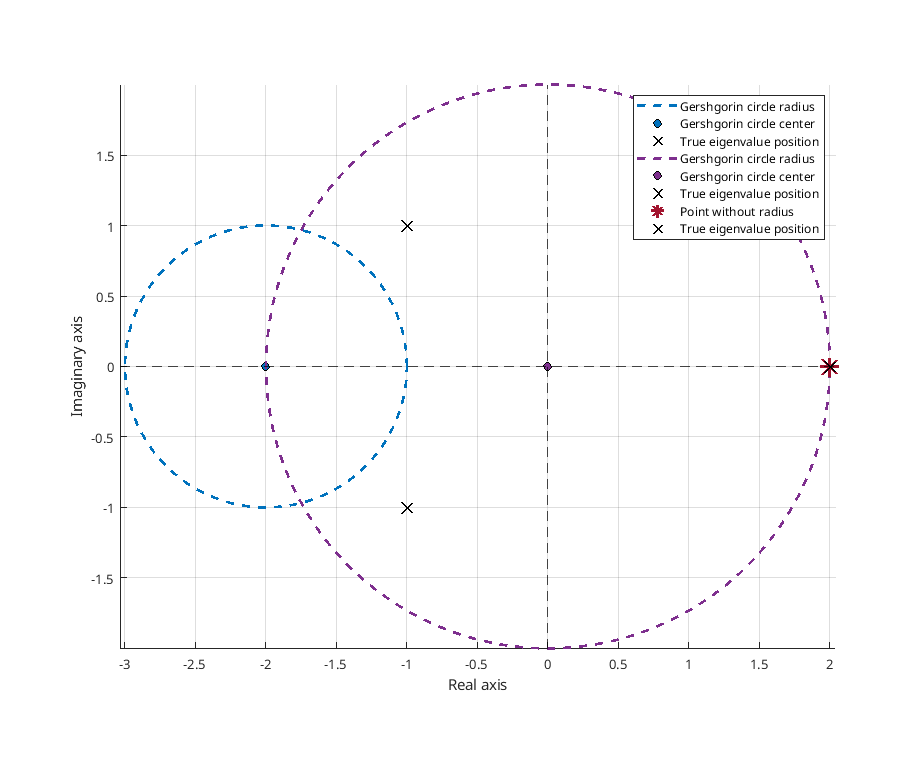
\includegraphics[width=1\textwidth]{problems/Figures/Problem_7/first_matrix.png}
    \caption{The Gershgorin disks and eigenvalues of the matrix $\matr{A}_1$.
    Please note, that the Gershgorin disk with the center in $-2$ does not contain any
    of the eigenvalues, which may be due to the matrix not being diagonally dominant.
    }
\end{figure}
\begin{figure}[H]
    \centering
    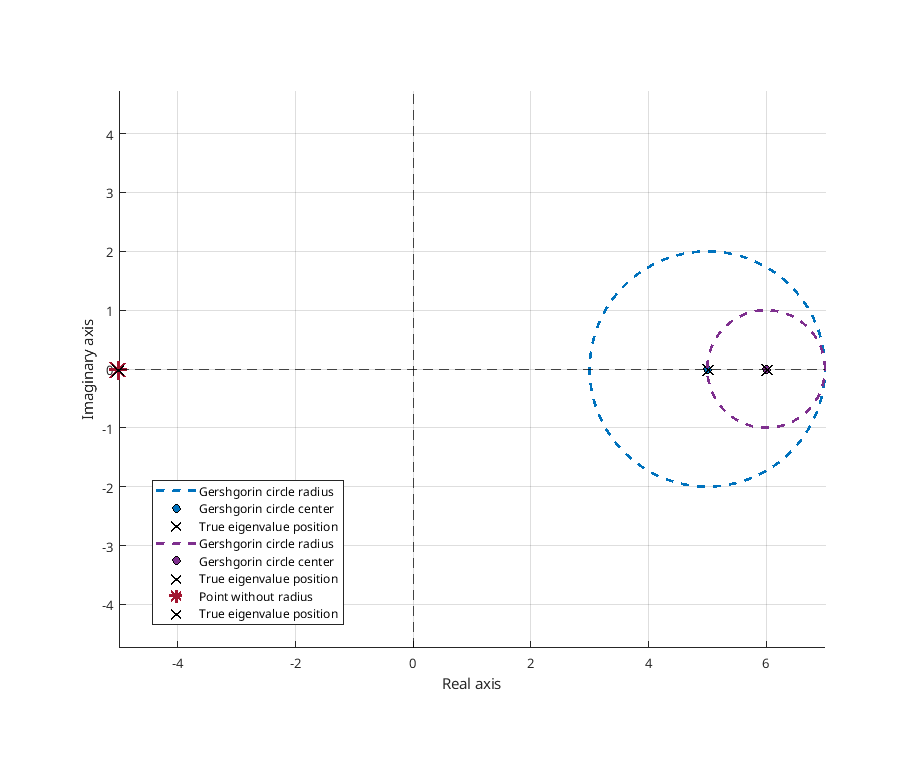
\includegraphics[width=1\textwidth]{problems/Figures/Problem_7/second_matrix.png}
    \caption{The Gershgorin disks and eigenvalues of the matrix $\matr{A}_2$.}
\end{figure}
\begin{figure}[H]
    \centering
    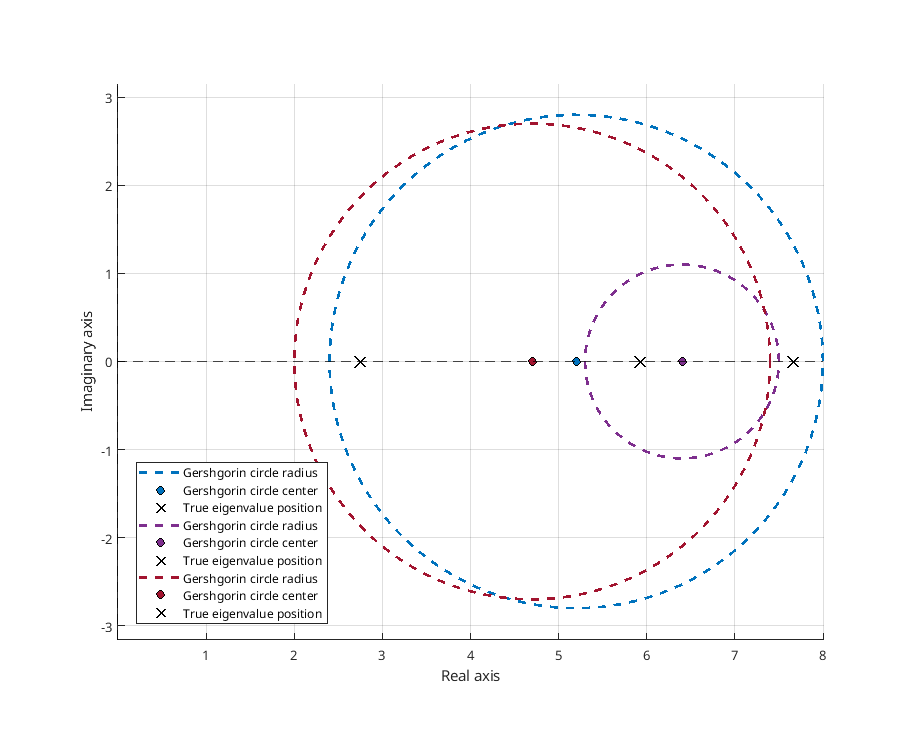
\includegraphics[width=1\textwidth]{problems/Figures/Problem_7/last_matrix.png}
    \caption{The Gershgorin disks and eigenvalues of the matrix $\matr{A}_3$.}
\end{figure}
